%\documentclass[iop]{emulateapj}
%\documentclass[12pt, preprint]{emulateapj}
\documentclass[12pt, onecolumn]{emulateapj}

\usepackage{tikz}
\usetikzlibrary{shapes.geometric, arrows}
\usetikzlibrary{fit}

\tikzstyle{hyper} = [rectangle, rounded corners, minimum width=1cm, minimum height=0.5cm,text centered, draw=black, fill=blue!30]
\tikzstyle{param} = [rectangle, rounded corners, minimum width=1cm, minimum height=0.5cm,text centered, draw=black, fill=green!30]
\tikzstyle{data} = [rectangle, rounded corners, minimum width=1cm, minimum height=0.5cm,text centered, draw=black, fill=red!30]
%\tikzstyle{hyper} = [trapezium, trapezium left angle=70, trapezium right angle=110, minimum width=1cm, minimum height=0.5cm, text centered, draw=black, fill=green!30]
%\tikzstyle{param} = [rectangle, minimum width=1cm, minimum height=0.5cm, text centered, draw=black, fill=green!30]
%\tikzstyle{data} = [diamond, minimum width=1cm, minimum height=1cm, text centered, draw=black, fill=red!30]
\tikzstyle{eqn} = [rectangle, minimum width=1cm, minimum height=0.5cm, text centered, draw=black]%, fill=green!30]
\tikzstyle{latent} = [diamond, minimum width=1cm, minimum height=0.5cm, text centered, draw=black]%, fill=green!30]
\tikzstyle{arrow} = [thick,->,>=stealth]

\newcommand{\myemail}{aimalz@nyu.edu}
\newcommand{\textul}{\underline}

\shorttitle{Probabilistic Redshift Distribution}
\shortauthors{Malz}

\begin{document}

\title{Probabilistic Redshift Distribution: Minimal Approach}

\author{A.I. Malz\altaffilmark{1}}
\altaffiltext{1}{CCPP}
\email{aimalz@nyu.edu}

\begin{abstract}
This paper answers the question of how one would calculate the redshift distribution function $\mathcal{N}(z)$ from a set of likelihood functions for the photometric redshifts of individual galaxies.
\end{abstract}

\keywords{photo-z}

\section{Introduction}

\section{Method}

\subsection{Probabilistic Model}

We would like to learn the redshift distribution function $\mathcal{N}(z)$ for a set of $J$ galaxies $j$.  We assume each galaxy has a known likelihood function $p(\vec{d}_{j}|z)$ for the observed data $\vec{d}_{j}$ (a set of magnitudes in each of several filters) over redshift $z$.  The full dataset of $\{\vec{d}_{j}\}_{j=1,\dots,J}$ will be denoted as $\textul{D}$.  The redshift distribution function may be expressed as Eq. \ref{eq:params}.

\begin{eqnarray}
\label{eq:params}
p(z|\mathcal{N}) &=& \mathcal{N}(z) \equiv \frac{\mathcal{N}|_{z}}{\int\mathcal{N}|_{z}dz}
\end{eqnarray}

The likelihood function for the redshift distribution function is given in Eq. \ref{eq:likelihood}, where the likelihoods for each galaxy's redshift are considered to be independent.  

\begin{eqnarray}
\label{eq:likelihood}
p(\textul{D}|\mathcal{N}) &=& \prod_{j=1}^{J}\int p(\vec{d}_{j}|z)\ p(z|\mathcal{N})dz
\end{eqnarray}

By Bayes' Rule, we may find the desired posterior according to Eq. \ref{eq:bayes}.  We want the posterior for direct comparison with prior work in the literature, but the likelihood of Eq. \ref{eq:likelihood} is in fact preferable.

\begin{eqnarray}
\label{eq:bayes}
p(\mathcal{N}|\textul{D}) &=& \frac{p(\textul{D}|\mathcal{N})p(\mathcal{N})}{p(\textul{D})}
\end{eqnarray}

It is generally considered difficult to calculate the posterior $p(\mathcal{N}|\textul{D})$ directly due to not knowing $p(\textul{D})$.  Instead, we may sample the desired distribution using Monte Carlo-Markov chain (MCMC) methods.  

\subsection{Fake Data}
\label{sec:fake}

We consider the $K=35$ redshift bins $B_{k}=[z^{B}_{k-1},z^{B}_{k}]$ for which \citet{she11} calculated posteriors for the redshift of each galaxy based on observations of the apparent magnitude in the five photmetric filters of SDSS.  We parametrize $\mathcal{N}(z)$ as a vector of histogram heights $\vec{\mathcal{N}}$ representing the probability that a galaxy's redshift lies within the corresponding bin.  Eq. \ref{eq:params} becomes Eq. \ref{eq:dparams}, although we actually work with the log of $\vec{\mathcal{N}}$ throughout.  

\begin{eqnarray}
\label{eq:dparams}
p(B_{k}|\vec{\mathcal{N}}) &=& \mathcal{N}_{k}% \vec{\mathcal{N}} \equiv \frac{\mathcal{N}_{k}}{\sum_{k=1}^{K}\mathcal{N}_{k}}
\end{eqnarray}

In order to simulate data, we set Eq. \ref{eq:truenz} as a true, physically motivated redshift function $\mathcal{N}^{0}$.  The convolution of a linear function and a sum of Gaussians is quite general and accurately generates features observed in the true $N(z)$.  (Cite this!)  We evaluate it at the center of each bin  $z_{k}=(z_{k+1}^{B}-z_{k}^{B})/2$ to obtain the discretized $\vec{\mathcal{N}}^{0}$.  Here we have defined $\bar{z}$ as the average redshift over the entire range $[z_{0},z_{K}]$.  Fig. \ref{fig:truenz} illustrates the construction of $\vec{\mathcal{N}}^{0}$.

\begin{mathletters}
\begin{eqnarray}
\label{eq:truenz}
\mathcal{N}^{0}' &=& \sum_{r=1}^{6}A_{r}\cdot N(z_{r},\sigma^{2}_{r})\nonumber\\
\mathcal{N}^{0} &=& \frac{\mathcal{N}^{0}'}{\int\mathcal{N}^{0}'dz}
%\frac{z_{k}^{z_{K}^{B}}\exp[-z_{k}*z_{1}^{B}]}{\sum_{k=0}^{K}z_{k}^{z_{K}^{B}}\exp[-z_{k}*z_{1}^{B}]}% N(\ln[\vec{\mu}],\textul{\Sigma})\\
%\mu_{k} &=& \frac{z_{k}^{z_{K}^{B}}\exp[-z_{k}*z_{1}^{B}]}{\sum_{k=0}^{K}z_{k}^{z_{K}^{B}}\exp[-z_{k}*z_{1}^{B}]}\nonumber\\
%\Sigma_{ij} &=& \left\{\begin{array}{cc}i=j&\ K^{-1/2}\\|i-j|=1&\ K^{-1}\\else&0\end{array}\right\}\nonumber
\end{eqnarray}
\end{mathletters}

\begin{figure}
\label{fig:truenz}
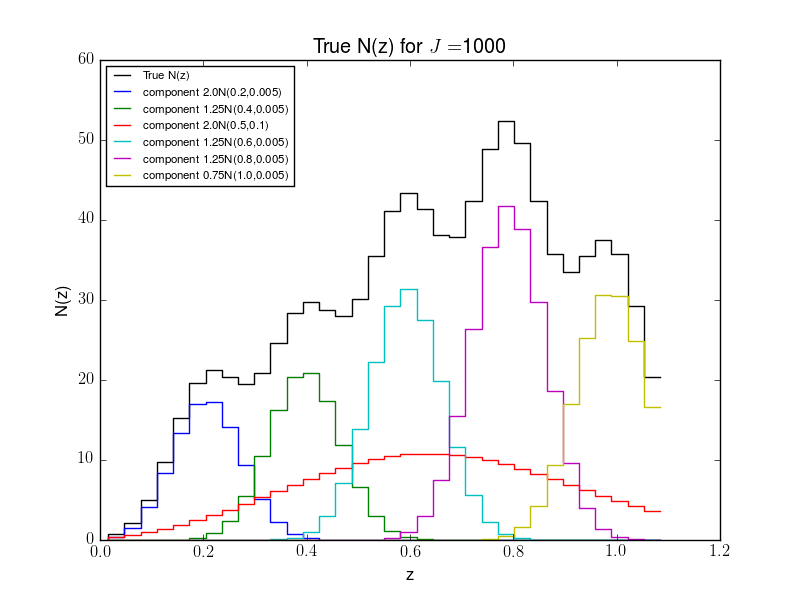
\includegraphics[scale=0.5]{trueNz.png}
\caption{We construct $\vec{\mathcal{N}}^{0}$ as a sum of Gaussians.}
\end{figure}

Next, we generate galaxy redshift likelihood functions as follows.  We first assign a bin number $b_{j}=k$ from $k=1,\dots,K$ to each of $J=1000$ galaxies by randomly sampling the $K$ bins with weights given by the true redshift function as $p(b_{j})\sim\mathcal{N}^{0}_{k}$.  Examples of some such samples for $J=1000$ galaxies are shown in Fig. \ref{fig:obsnz}.

\begin{figure}
\label{fig:obsnz}
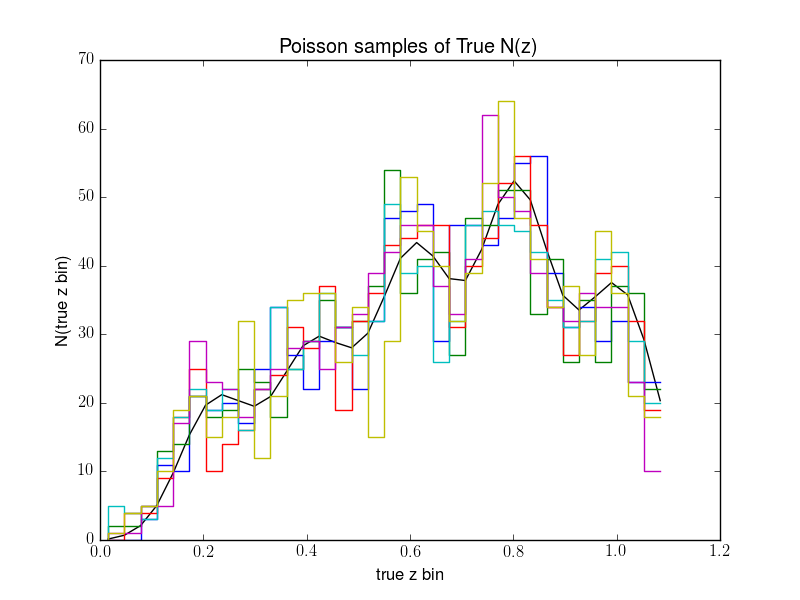
\includegraphics[scale=0.5]{obsNz.png}
\caption{Samples of the true redshift function are generated as Poisson draws.}
\end{figure}

We then assign each galaxy a true redshift $z_{j}$ chosen uniformly from within the bin $B_{b_{j}}$ to which it was assigned.  Here it is convenient to define $\beta$ as the mean redshift per bin.  The true redshift of each galaxy is shifted by a random error according to Eq. \ref{eq:zshift} to simulate inaccuracy in measurements, yielding a shifted redshift $z_{j}'$ for each galaxy.  Fig. \ref{fig:samples} shows histograms of the fake data generated.  It is worth noting that any method aiming to calculate the posterior can do no better than the ``observed redshifts'' that go into generating the data.

\begin{mathletters}
\begin{eqnarray}
\label{eq:zshift}
z_{j}' &=& z_{j}+e_{j}\\
p(e_{j}) &=& N(0,\delta_{j})\nonumber\\
\delta_{j} &=& \frac{\sum_{b_{k}=1}^{K}(z_{b_{k}}-z_{b_{k}-1)}}{K}(1+z_{j})\nonumber
\end{eqnarray}
\end{mathletters}

\begin{figure}
\label{fig:samples}
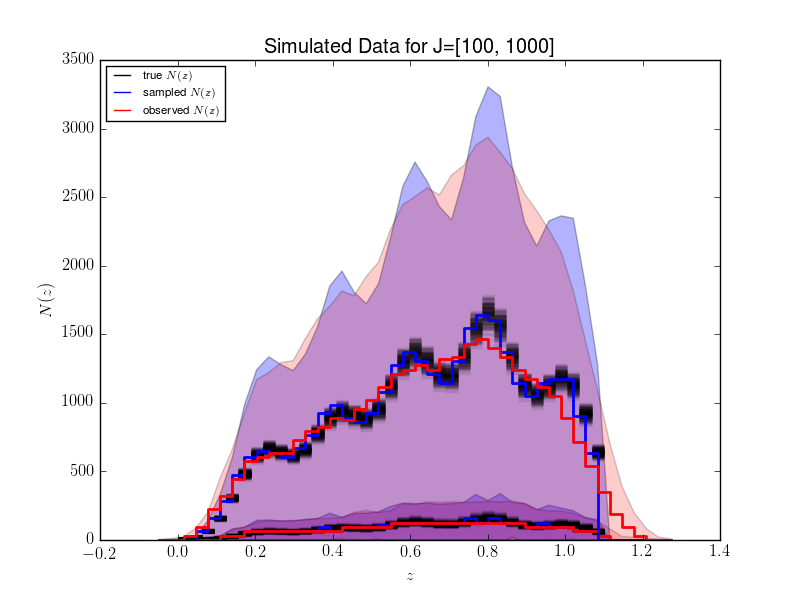
\includegraphics[scale=0.5]{simdata.png}
\caption{The true $\vec{\mathcal{N}}$ chosen for this test is plotted here, along with histograms of the true redshifts sampled from it and the shifted redshifts resulting from the fake data generation procedure.}
\end{figure}

The discretized likelihood function $p(\vec{d_{j}}|B_{k})$ for each galaxy is taken to be Gaussian with a mean equal to the shifted redshift and a standard deviation proportional to one plus the true redshift to simulate the fact that uncertainty increases with redshift.  According to the above, "the data" are thus comprised of $J$ pairs $(z_{j}',\delta_{j})$.  Thus the observed probability that galaxy $j$ has a redshift in bin $k$ is given by Eq. \ref{eq:zdist}.  As a final step, all likelihoods are normalized such that they sum to unity over the redshift range spanned by the bins.  Fig. \ref{fig:pzs} shows a few examples of simulated likelihoods.

\begin{eqnarray}
\label{eq:zdist}
\mathcal{L}_{j}^{k} &\equiv& p(\vec{d_{j}}|B_{k}) = \int_{z_{k-1}}^{z_{k}} \frac{1}{\sqrt{2\pi\delta_{j}^{2}}}\exp\left[-\frac{(z_{j}'-\tilde{z})^{2}}{2\delta_{j}^{2}}\right]d\tilde{z}
\end{eqnarray}

\begin{figure}
\label{fig:pzs}
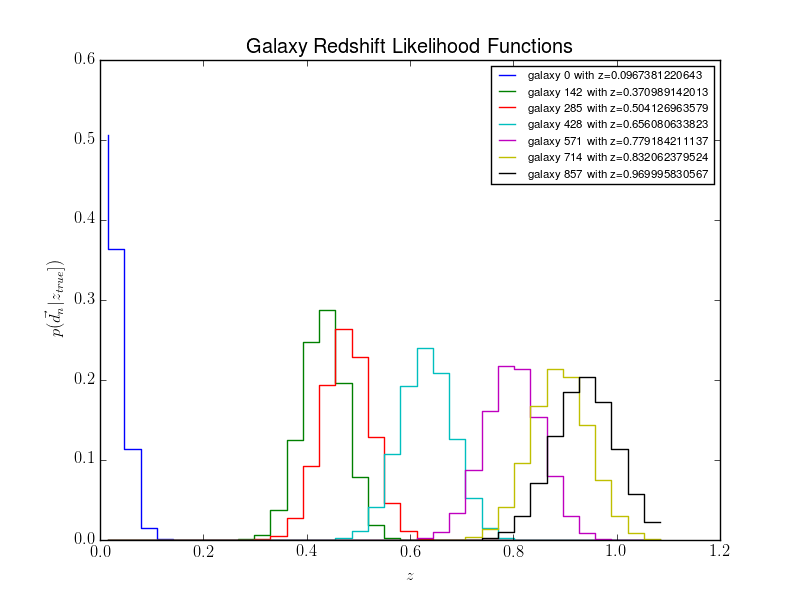
\includegraphics[scale=0.5]{lik-samps.png}
\caption{Several random redshift likelihood functions are shown here.  Note that the width of the Gaussian increases with redshift.}
\end{figure}

\section{Results}

The Metropolis-Hastings algorithm is applied to sample the posterior.  The procedure is initialized with the log of the average probability (i.e. a flat distribution), which shall be denoted $\ln\vec{\mathcal{N}}\equiv\ln p(z|\vec{\mathcal{N}})$.  The log of the numerator of the posterior of Eq. \ref{eq:bayes} is calculated according to Eq. \ref{eq:disc-post} and is denoted as $\ln\tilde{p}(\vec{\mathcal{N}}|\textul{D})$.  

Samples are generated from a multivariate normal with the covariance matrix of Eq. \ref{eq:covmat}.  This covariance structure is chosen to enforce continuity of the histogram heights.  Some examples of samples from the initialization value are shown in Fig. \ref{fig:priors}.

\begin{mathletters}
\begin{eqnarray}
\label{eq:covmat}
p(\ln\vec{\mathcal{N}}') &=& N(\ln[\vec{\mathcal{N}}],\textul{\Sigma})\\
\Sigma_{ij} &=& q\cdot e^{a(i-j)^{2}/2}\nonumber
\end{eqnarray}
\end{mathletters}

\begin{figure}
\label{fig:priors}
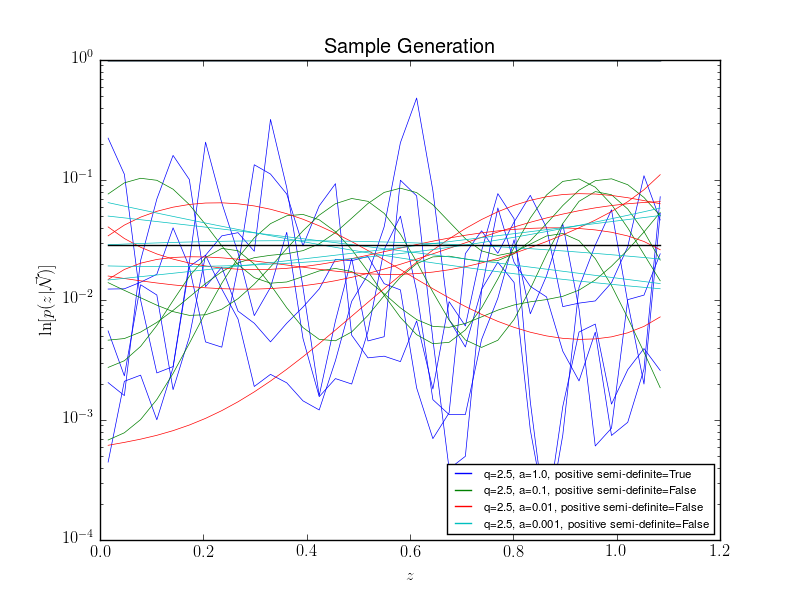
\includegraphics[scale=0.5]{sampgen.png}
\caption{Several random samples of $\vec{\mathcal{N}}$ from the distribution of Eq. \ref{eq:covmat} are shown here.  The covariance matrix with $a=1$ is the only one of this structure that is positive semi-definite, but other values of $a$ lead to smoother samples.}
\end{figure}

The following pseudo-code outlines the algorithm.

\begin{enumerate}
\item \label{it:randsamp} Randomly sample Eq. \ref{eq:covmat} to generate a proposal $\ln\vec{\mathcal{N}}'$.
\item Calculate the log of the numerator of the posterior as in Eq. \ref{eq:disc-post} to produce $\ln\tilde{p}(\vec{\mathcal{N}}'|\textul{D})$.
\item Calculate $r=\ln\tilde{p}(\vec{\mathcal{N}}'|\textul{D})-\ln\tilde{p}(\vec{\mathcal{N}}|\textul{D})$.
\item If $r\geq0$, set and record $\ln\vec{\mathcal{N}}=\ln\vec{\mathcal{N}}'$; recalculate $\ln\tilde{p}(\vec{\mathcal{N}}|\textul{D})$.\\
If $r<0$, select a random number $n$ from the uniform distribution between 0 and 1.
\begin{enumerate}
\item If $n<e^{r}$, set and record $\vec{\mathcal{N}}=\vec{\mathcal{N}}'$; recalculate $\ln\tilde{p}(\vec{\mathcal{N}}|\textul{D})$.
\end{enumerate}
\item Check if the threshold has been achieved; if not, return to Step \ref{it:randsamp}.
\end{enumerate}

\begin{eqnarray}
\label{eq:disc-post}
\ln\tilde{p}(\vec{\mathcal{N}}'|\textul{D}) &\equiv& \ln p(\vec{\mathcal{N}}) + \sum_{j=1}^{J}\ln\left[\sum_{k=1}^{K}p(\vec{d}_{j}|z_{k})\ p(z_{k}|\vec{\mathcal{N}})\right] \propto \ln p(\vec{\mathcal{N}}|\textul{D})\\
\ln p(\vec{\mathcal{N}})_{k} &=& N(K^{-1},\textul{\Sigma})\nonumber\\
\Sigma_{ij} &=& \left\{\begin{array}{cc}i=j&\ 1\\|i-j|=1&\ \frac{1}{2}\\else&0\end{array}\right\}
\end{eqnarray}

Here, the threshold was stability up to an arbitrary $R=1000$ iterations of the algorithm.  All accepted proposals from one instance of the code are shown in Fig. %\ref{fig:results}
.  The acceptance fraction was $\sim0.1\%$ for this and other runs.  Since 10000 iterations likely doesn't even get through the ``burn-in'' period of the algorithm, this acceptance fraction is not surprising!  If I were convinced it were otherwise valid, I would run it until some convergence criterion were achieved.  However, since that might take quite some time, I will conservatively refrain from doing so.

%\begin{figure}
%\label{fig:results}
%\includegraphics[scale=0.75]{compare-results.png}
%\caption{Accepted proposal values of $\vec{\mathcal{N}}$ are shown here, along with the true value in black.}
%\end{figure}

\section{Discussion}

It is desirable to compare this result to what would have been obtained by the method of \citet{she11}, which directly calculates the posterior for the entire dataset using the posteriors for each galaxy according to Eq. \ref{eq:sheldon}.

\begin{eqnarray}
\label{eq:sheldon}
p(B_{k}|\vec{\mathcal{N}}) &=& \sum_{n=1}^{N}p(B_{k}|\vec{d}_{j})
\end{eqnarray}

To do this, I calculate the posteriors $p(z|\vec{d}_{j})$ for each galaxy using Eq. \ref{eq:posts}, the product of the estimate of $\vec{\mathcal{N}}$ and the likelihood for each galaxy.  This is done for all accepted values of $\vec{\mathcal{N}}$.

\begin{eqnarray}
\label{eq:posts}
p(B_{k}|\vec{d}_{j}) &=& p(\vec{d}_{j}|B_{k})p(\vec{\mathcal{N}}|\textul{D})
\end{eqnarray}

Fig. \ref{fig:sheldon} compares the result of summing the posteriors as in Eq. \ref{eq:sheldon} with the result of the MCMC solutions of Eq. \ref{eq:bayes}.  The method of \citet{she11} underestimates the probability of observing low redshifts.  As one would expect, the MCMC estimate irreversibly loses some substructure because of the shifting error added to the simulated data.

\begin{figure}
\label{fig:sheldon}
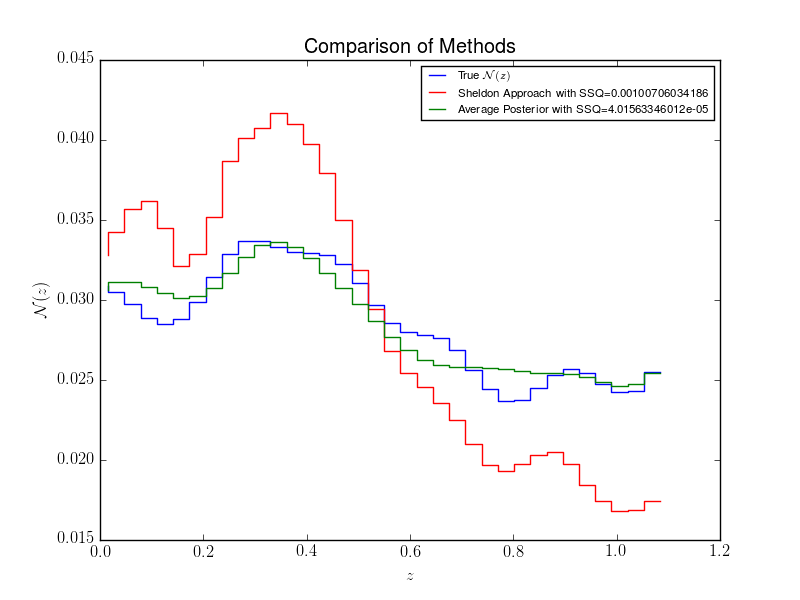
\includegraphics[scale=0.5]{compare-sheldon.png}
\caption{The result of applying Eq. \ref{eq:sheldon} is shown in red, the average accepted posterior sample from the method presented here is shown in blue, and $\mathcal{N}(z)$ for the observable redshifts of Eq. \ref{eq:zshift} is shown in black.  The sum of squared differences between the result of each method and the true value are also shown; one can see that the \citet{she11} approach has larger errors.}
\end{figure}

%\acknowledgments

%\appendix

\begin{thebibliography}{}
\bibitem[Benitez (2000)]{ben00}
Benitez, N., ApJ 536:571-̀583, 2000 June 20
\bibitem[Cunha, et al. (2008)]{cun08}
Cunha, C.E., Lima, M., Oyaizu, H., Frieman, J., Lin, H., arxiv:0810.2991
\bibitem[Fadely, et al. (2012)]{fad12}
Fadely, R., Hogg, D.W., Willman, B., arxiv:1206.4306
\bibitem[Foreman-Mackey, Hogg, and Morton (2014)]{for14}
Foreman-Mackey, D., Hogg, D.W., and Morton, T.D., arxiv:1406.3020
\bibitem[Hogg (1999)]{hog99}
Hogg, D.W., arxiv:astro-ph/9905116
\bibitem[Hogg, et al. (2010)]{hog10}
Hogg, D.W., Myers, A.D., Bovy, J., arxiv:1008.4146
\bibitem[Hogg (2012)]{hog12}
Hogg, D.W., arxiv:1205.4446
\bibitem[Lima, et al. (2008)]{lim08}
Lima, M., Cunha, C.E., Oyaizu, H., Frieman, J., Lin, H., Sheldon, E.S., MNRAS, 390, 118
\bibitem[Sheldon, et al. (2011)]{she11}
Sheldon, E.S., Cunha, C., Mandelbaum, R., Brinkmann, J., Weaver, B.A., arxiv:1109.5192

FILL IN MORE OF THESE!
\end{thebibliography}

\end{document}